\begin{abstract}
	Le dimensionnement de lots est un problème classique en planification de production. Différents critères \cite{cathy} permettent de classifier les problèmes de dimensionnement de lots. Suivant les classifications proposées, différentes classes peuvent être identifiées au nombre desquelles on peut citer le \emph{Discrete Lot Sizing Problem} (DLSP) dont le PSP fait partie. Différentes méthodes et modèles ont ainsi été appliqués au PSP \cite{ratheil_master} \cite{ceschia} avec différents résultats.
\end{abstract}

\section*{Introduction}
	\addcontentsline{toc}{section}{Introduction}
		
		Dans ce chapitre, nous présentons la revue de littérature des problèmes de dimensionnement de lots en planification de production dont fait parti le PSP. Nous exposons les méthodes de recherche déjà appliquées dans la résolution du PSP et soulignons les travaux effectués sur les algorithmes génétiques. Nous montrons également en quoi les algorithmes génétiques pourraient être particulièrement adaptés à ce genre de problèmes.
		
	\section{Le dimensionnement de lots en planification de production}
	La planification de production est un processus qui consiste à déterminer un plan qui indique quelle quantité d'articles produire durant un intervalle de temps appelé "horizon de planification". La planification de production occupe donc une place stratégique en industrie aussi bien en terme de performance que de coûts d'exploitation.\\
	\hspace*{.5cm} Différentes recherches \cite{dauzere} ont été menées dans le but de classifier les problèmes de dimensionnement de lots. Plusieurs critères ont pu être identifiés. Nous présentons dans cette section quelques critères de classification \cite{cathy} des problèmes de dimensionnement de lots.
	
\subsection{Critères de classification}

Différents critères interviennent dans la classification des problèmes de dimensionnement de lots, notamment : 
\begin{description}
	\item[\textsl{L'échelle de temps}:] L'horizon de planification peut être soit discret ou continu. Lorsqu'il est discret, on distingue alors les problèmes de petite taille ou \emph{Small time buckets}, les problèmes de grande taille ou \emph{Big time Buckets} et enfin les problèmes de très grandes taille ou \emph{Very big time buckets}.

	\item[\textsl{Le nombre de niveaux}:] Suivant qu'une relation ou non soit définie entre les articles, on distingue les problèmes à un niveau et les problèmes à plusieurs niveaux. Dans les problèmes à plusieurs niveaux, la production d'un article est conditionnée par celle d'un autre article. 

	\item[\textsl{Le nombre de produits}:] Un problème peut être qualifié soit de \emph{multi-item} (plusieurs types d'articles) ou de \emph{single-item} (un unique type d'articles). Il est \emph{multi-item} lorsque plusieurs types d'articles sont produits et \emph{single-item} dans le cas d'un unique type d' articles produit. 

	\item[\textsl{Les contraintes de capacité}:] Les contraintes de capacité sont diverses. Elles peuvent concerner aussi bien la capacité de stockage, la capacité des machines, etc. La prise en compte de ces contraintes de capacité rend le problème plus complexe à résoudre.

	\item[\textsl{Les demandes}:] Les demandes peuvent être aussi bien:
	\begin{itemize}
		\item[•] constantes avec des valeurs qui ne changent pas sur l'horizon de temps ou dynamiques avec  des valeurs qui sont fonction du temps.
		\item[•] certaines avec des valeurs connues à l'avance sou stochastiques avec des valeurs basées sur des probabilités.
		\item[•] indépendantes sans lien entre les articles à produire ou dépendantes en cas de relation entre articles.
	\end{itemize}

	\item[\textsl{Les coûts et temps de lancement ou préparation (setup)}:] Ils sont induits en cas de changement de types d'articles produits au cours d'un horizon de planification. On parle alors de transition.
	
\end{description}

	Nous avons choisi dans cette étude de décrire les problèmes de dimensionnement de lots selon la longueur de la période de l'horizon de temps. Nous allons donc nous intéresser aux problèmes à courtes et longues périodes.
\subsection{Classes de problèmes de dimensionnement de lots}
	\subsubsection{Problèmes à courtes périodes}
	Ces problèmes (\emph{Small time bucket problems}) sont caractérisés par des périodes de l'ordre de quelques heures, et la séquence des lots lors de la production est prise en compte. Quatre types de problèmes sont étudiés dans la littérature. Ces différents types de problèmes sont donc:
	\begin{description}
		\item[\textsl{Discrete lot-sizing and scheduling problem (DLSP):}] Dans ce problème \cite{fleischmann}, au plus un article peut être produit par période. Dans le cas où un article est produit sur une période, alors toute la capacité disponible sur cette période sera utilisée. Les coûts de lancement sont en général pris en compte seulement lorsqu'un nouveau lot commence et non à chaque période.
		\item[\textsl{Continuous setup lot-sizing problem (CSLP):}]
		Le CSLP reprend les mêmes principes que le problème précédent à la seule différence que lorsqu'un article est produit, ce n'est plus toute la capacité qui est utilisée mais uniquement la capacité nécessaire à la production.
		\item[\textsl{Proportional lot-sizing and scheduling problem (PLSP):}] 
		Dans ce problème, la capacité restante pour une période donnée est réutilisée pour produire un second article. Le cas à plusieurs niveaux et plusieurs machines représente par exemple, une extension de ce problème. 
		\item[\textsl{General lot-sizing and scheduling problem (GLSP):}] 
		Dans ce problème \cite{fleischmann_meyr}, Aucune restriction n'est appliquée sur le nombre d'articles à produire par période. En intégrant des temps de lancement de production dépendants de la séquence des lots à produire, on obtient des extensions du GLSP \cite{meyr}.
	\end{description}
	
	\subsubsection{Problèmes à longues périodes}
	Dans les problèmes de grande taille (\emph{Big time bucket problems}), l'horizon va de quelques jours à quelques semaines. De même, un produit peut être fabriqué par période. Nous proposons dans cette section, une étude concise de ces problèmes.
	
	\begin{description}
		\item[Les problèmes à un niveau et un produit]: \\
		Manne \cite{manne} et Wagner et Whitin \cite{wagner_whitin} ont été à l'initiative sur l'étude de cette classe de problèmes. Ils ont permis la mise au point d'une méthode de résolution utilisée afin de résoudre des problèmes plus complexes. En effet, la résolution des problèmes à plusieurs niveaux bénéficie grandement des méthodes mises en œuvre dans la résolution des problèmes à un niveau et un produit.
				
		\item[Les problèmes à un niveau et plusieurs produits]: \\
		Ces problèmes introduisent des contraintes de capacité qui s'accompagnent d'une relation entre les différents articles produits, rendant ainsi le problème plus difficile à résoudre.
		
		\item[Les problèmes à plusieurs niveaux]: \\ 
		Une des principales caractéristiques de ces problèmes est le fait que les produits intermédiaires entrent dans la production des produits finis. Ainsi, les demandes entre les produits ou demandes dépendantes et les demandes indépendantes que sont demandes arrivant de l'extérieur sont prises en compte dans ce type de problème.
		
	\end{description}
	
	Un exemple d'un problème de "\emph{Big time bucket}" est le cas où différents articles peuvent être produit sur une même ressource en une seule période. Ce problème est connu sous le nom de "Capacited Lot Sizing Problem" (CLSP). Le CLSP consiste à déterminer le coût et le temps de production des articles dans l'horizon de planification. La figure \ref{fig:classification_dimensionnement_lots} présente un exemple de classification des modèles de dimensionnement de lots.
	
	\begin{center}
		\begin{figure}[!h]
			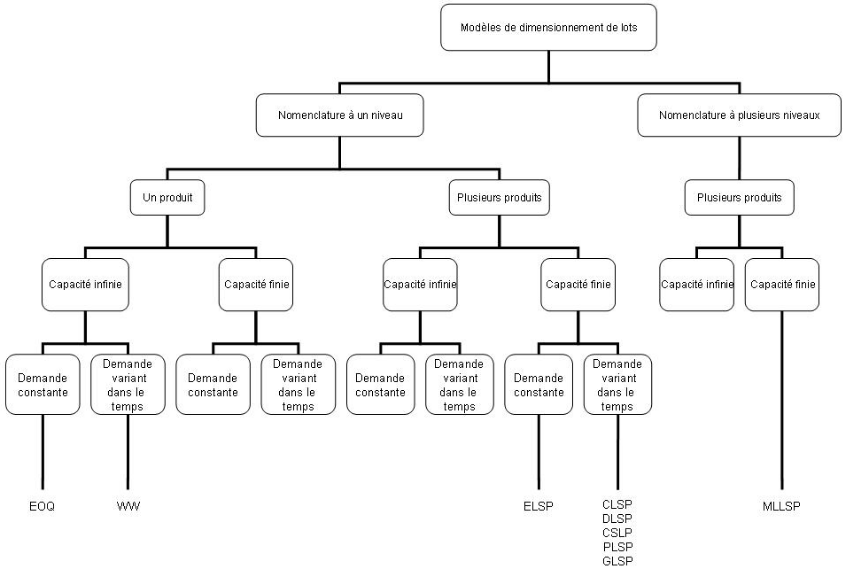
\includegraphics[scale=.5]{images/classification_dimensionnement.png}
			\caption{Exemple de classification des modèles de dimensionnement de lots \cite{cathy}}
			\label{fig:classification_dimensionnement_lots}
		\end{figure}
	\end{center}

	\newpage
	
	\section{Le \emph{Pigment sequencing problem} (PSP)}
	
	\subsection{Revue de littérature}
	Le PSP appartient à la catégorie des DLSP. En effet, il s'agit d'un problème où toute la capacité disponible sur cette période sera utilisée si un article est fabriqué. Nous présentons dans cette section une brève revue de littérature des différents travaux effectués autour du PSP. \\
	\hspace*{.5cm} Miller et Wolsey \cite{miller_wolsey} ont formulé le DLSP avec des coûts de préparation indépendants de séquence comme un problème de réseau à flot. Ils ont présenté des formulations MIP pour les différentes extensions (avec \emph{backlogging}, avec stock de sûreté, avec stock initial). Plusieurs variantes et formulations MIP du DLSP ont été proposées et discutées par Pochet et Wolsey \cite{pochet_wolsey}. \\
	\hspace*{.5cm} Gicquel et al. \cite{gicquel_minoux_dallery} présentent une formulation et dérivent des inégalités valides pour le DLSP avec plusieurs articles et des coûts et temps de préparation séquentiels; laquelle est une extension du problème proposé par Wolsey \cite{wolsey}. Dans Gicquel et al. \cite {gicquel_miegeville_minoux_dallery}, les auteurs ont proposé une nouvelle manière de modéliser le DLSP avec plusieurs articles et des coûts et temps de préparation séquentiels; qui exploite le fait que les attributs physiques pertinents des articles, tels que la couleur, la dimension, le niveau de qualité. Cela leur a permis de réduire significativement le nombre des variables et des contraintes dans les modèles MIP.\\
	\hspace*{.5cm}Houndji et al. \cite{hvr_stockingCost} ont introduit une nouvelle contrainte globale, qu'ils ont appelée \emph{StockingCost} afin d'efficacement résoudre le PSP en programmation par contrainte. Les auteurs l'ont alors testée sur de nouvelles instances et les ont publiées sur CSPlib (Gent et Walsh \cite{gent_walsh}). Les résultats expérimentaux ont montré que le \emph{StockingCost} est plus efficace en filtrage par rapport aux autres contraintes généralement utilisées dans la communauté de la programmation par contrainte. \\
	\hspace*{.5cm} Plus récemment, Ceschia et al. \cite{ceschia} ont appliqué le recuit simulé sur le PSP. Ils ont introduit une procédure de recuit simulé afin de guider la recherche locale, qu'ils ont ensuite appliquée sur de nouvelles instances disponibles sur le bibliothèque Opthub \cite{opthub}.
	 
	\subsection{Description du problème}{\label{sec:problem_description}}

		Des différentes études \cite{ratheil_master} \cite{ceschia} déjà effectuées sur le PSP, nous pouvons le décrire comme une problème qui consiste à trouver un plan de production de plusieurs articles à partir d’une machine avec des coûts de transition. Les coûts de transition sont les coûts encourus lors du passage de la production de l’article $i$ à celui de l’article $j$ avec $i \neq j$. Le plan de production doit satisfaire les demandes des clients tout en :
	\begin{itemize}
		\item[•] respectant la capacité de production de la machine;
		\item[•] minimisant les coûts de stockage et de transition.
	\end{itemize}
	\hspace*{.5cm} On suppose que la période de production est suffisamment courte pour ne produire qu’au plus un article par période et que les demandes sont normalisées : la capacité de production de la machine est limitée à un article par
période et d($i$, $t$) $ \in $ {0, 1} avec $i$ l’article et $t$ la période.\\
	\hspace*{.5cm} Il s’agit d’un problème de planification de production ayant les caractéristiques suivantes : un horizon de planification discret et fini ; des contraintes de capacité ; une demande statique et déterministe ; multi-item et small bucket, des coûts de transition; un seul niveau; sans shortage.\\

	\textbf{\textsl{Illustration}} : Soit un problème avec les données ci-dessous : \\
	\begin{itemize}
		\item[•] Nombre d’articles : $NI = 2$;
		\item[•] Nombre de périodes : $NT = 5$;
		\item[•] Demande par période. Soit d($i$, $t$) la demande de l’article $i$ à la période $t$ : $d(1, t) = (0, 1, 0, 0, 1)$ et $d(2, t) = (1, 0, 0, 0, 1)$;
		\item[•] Coût de stockage. Soit $h(i)$ le coût de stockage de l’article $i$ : $h(1) = h(2) = 2$;
	\end{itemize}
	Soit \emph{xT} le plan de production qui représente une solution potentielle du problème. Il s’agit d’un tableau de dimension \emph{NT} , contenant à son indice $t$ (avec $t  \in  {1...NT}$) l’article $i$ à produire. Une solution admissible du problème est : $ xT = (2, 1, 2, 0, 1)$ avec un coût de $ q(2, 1) + q(1, 2) + q(2, 1) + 2 * h(2) = 15 $. La solution optimale est : $ xT = (2, 1, 0, 1, 2)$ avec un coût de $q(2, 1) + q(1, 2) + h(1) = 10$.
		
		\subsection{Modèles et formulations}
		Différents modèles ont été proposés afin de représenter, modéliser et résoudre le PSP. Il s'agit des modèles de programmation mixte en nombres entiers ou MIP (au nombre de 3) proposés par Pochet et Wolsey \cite{pochet_wolsey}, considérés comme l'état de l'art des méthodes de résolution exactes sur les problèmes de dimensionnement de lots en particulier celui du PSP, du modèle CP et du modèle SA. Nous présentons donc ici le premier modèle MIP dont les deux derniers sont une reformulation, le modèle CP ainsi que le modèle SA.
		\subsubsection{Modèle MIP 1}
		
		Le modèle MIP 1 \cite{pochet_wolsey} tel qu'exposé par Pochet et Wolsey se présente comme suit:
		\begin{eqnarray}
			min \sum_{i,j,t} q^{i,j}\chi_{t}^{i,j} + \sum_{i,t} h^{i} s_{t}^{i} \\
			s_{0}^{i} = 0, \forall i \\
			x_{t}^{i} + s_{t-1}^{i} = d_{t}^{i} + s_{t}^{i}, \forall i,t \\
			x_{t}^{i} \leq y_{t}^{i}, \forall i,t \\
			\sum_{i} y_{t}^{i} = 1 , \forall t \\
			\chi_{t}^{i,j} = y_{t-1}^{i} + y_{t}^{j} - 1, \forall i,j,t \\
			x,y,\chi \in \{0,1\}, s \in \mathbb{N}, i \in \{0..NI\}, t \in \{1..NT\}
		\end{eqnarray}
		
		avec les variables de décisions suivantes: \\
		\begin{itemize}
			\item[-] $x_{t}^{i}$ : variable binaire de production qui vaut 1 si l’article $i$ est produit à la période $t$ et 0 sinon ;
			\item[-] $y_{t}^{i}$ : variable binaire de setup qui vaut 1 si la machine est préparée pour la production de l’article $i$ et 0 sinon ;
			\item[-] $s_{t}^{i}$ : variable entière de stockage qui contient le nombre d’articles $i$ stockés à la période $t$ ; 
			\item[-] $\chi_{t}^{i,j}$ : variable binaire de transition qui vaut 1 si à la période $t$, on est passé de la production de l’article $i$ à l’article $j$ et 0 sinon.
		\end{itemize}
		\vspace*{.3cm}
	\hspace*{.5cm} L'objectif est de minimiser la somme des coûts de stockage et des coûts de transition et est exprimé par la contrainte (1). La contrainte (2) rappelle qu'il n'y a pas de stock initial. La contrainte (3) exprime la règle de la conservation de flot. La contrainte (4) vise à forcer la variable de setup $y_{t}^{i}$ à prendre la valeur 1 s’il y a production de l’article $i$ à la période $t$. La contrainte (5) s'assure qu'il y a toujours un article qui est préparé. En accord avec la fonction objectif, $y_{t}^{i}$ va prendre la valeur qui minimise le coût de transition. En général s’il n’y a pas de production à la période $t$,
$y_{t}^{i} = y_{t-1}^{i}$ ou $y_{t}^{i} = y_{t+1}^{i}$
mais parfois il peut être intéressant de préparer la machine pour un article intermédiaire sans le produire. La contrainte (6) assigne les valeurs aux variables de transition.
En effet, si $y_{t-1}^{i}$ et $y_{t}^{i}$ valent 1 alors $\chi_{t}^{i,j}$ est obligé de prendre la valeur 1 et sinon $\chi_{t}^{i,j}$ serait égale à 0 grâce à la fonction objectif qui minimise le coût de transition.
		
		\subsubsection{Modèle CP}
		Dans ce modèle \cite{ratheil_master}, l’objectif est d’attribuer à chacune des demandes, une période qui respecte la date limite de satisfaction de la demande. On note $date(p) \in [1,...,T],\ \forall p \in [1,...,n]$ la période dans laquelle la demande $p$ a été satisfaite, $dueDate(p) \in [1,...,T]$ la date limite de la demande $p$ et $I(p)$ l'article correspondant à la demande $p$. Afin de s'assurer de la faisabilité de la solution, les principales contraintes sont les suivantes:
		\begin{eqnarray}
			date(p) \leq duedate(p), \forall p \\
			alldifferent(date)
		\end{eqnarray}
		
		dans lesquelles:
		\begin{itemize}
			\item[-] Equation 8: chaque demande doit être satisfaite avant sa date limite;
			\item[-] Equation 9: Puisque la capacité d'une machine est limitée à 1, chaque demande doit être satisfaite à différente période.
		\end{itemize}
		Il est possible de modéliser la partie des coûts de transition comme un ATSP, chaque demande représente une ville qui doit être visitée et les coûts de transition sont les distances entre deux villes. Ainsi, on ajoute une demande artificielle $n+1$ de sorte que $date(n+1) = T+1$ avec $q^{I(p), I(n+1)} = q^{I(n+1), I(p)} = 0, \forall p \in [1,...,n]$. On note alors $successor(p), \forall p \in [1,...,n]$, la demande satisfaite juste après la satisfaction de la demande $p$. Les contraintes suivantes additionnelles peuvent être alors ajoutées:
		\begin{eqnarray}
			circuit(successor) \\
			date(p) \leq date(successor(p)), \forall p \in [1,...,n]
		\end{eqnarray}
		dans lesquelles:
		\begin{itemize}
			\item[-] Equation 10: il garantit l'existence d'un circuit hamiltonien;
			\item[-] Equation 11: la demande $p$ doit être satisfaite avant ses successeurs.
		\end{itemize}
		
		Enfin, l'objectif est de minimiser les coûts de stockage et les coûts de transition.
		\[
			\sum_{p}{(dueDate(p)-date(p))} * h_{I(p)} + \sum_{p}{q^{I(p),I(successor(p))}}
		\]
		
	
		\subsubsection{Modèle SA}
		Dans ce modèle \cite{ceschia}, la procédure de recuit simulé conduit à chaque itération à une action aléatoire en utilisant une distribution uniforme. En recuit simulé, l'action est toujours acceptée si elle est facteur d'amélioration. Dans le cas contraire, elle est acceptée, si elle est basée sur une distribution en temps croissant de façon exponentielle. Dans le détail, une mauvaise action est acceptée avec une probabilité de $e^{-\Delta/T}$ où $\Delta$ est la différence du coût total induit par l'action et $T$ est la température. La température commence à une valeur $T_{0}$ et est multipliée par $\alpha$ (avec $0 < \alpha < 1$), après un nombre fixé d'échantillons $n_{s}$, selon la procédure de refroidissement géométrique standard du recuit simulé. \\
		\hspace*{.5cm} Dans le but d'accélérer les premières étapes de la procédure de recuit simulé,  Ceschia et al. ont utilisé un mécanisme de \emph{cut-off} (Johnson et al. \cite{johnson}). Ils ont ajouté un nouveau paramètre $n_{a}$ représentant le nombre maximal d'actions acceptées à chaque niveau de température. Ainsi, la température diminue lorsque la première des deux conditions suivantes est remplie : ($i$) le nombre d'actions échantillonnées atteint $n_{s}$, ($ii$) le nombre d'actions acceptées atteint $n_{a}$. \\
		\hspace*{.5cm} Le critère de terminaison est basé sur le nombre total d'itérations $I_{max}$, plutôt que sur un seuil de température. De cette manière, le temps d'exécution est approximativement le même pour toutes les configurations des paramètres.
		
	\section{Les algorithmes génétiques}
		
	Les algorithmes génétiques sont des algorithmes qui tirent leur origine de l'analogie avec l'évolution naturelle des espèces vivantes et des mécanismes de reproduction. Ils ont été proposés pour la première fois par John Holland \cite{holland1} en 1970. Un des principes fondamentaux des algorithmes génétiques est celui de la survie du "mieux adapté". Selon ce principe, un individu avec des caractéristiques en adéquation avec le milieu dans lequel il évolue à beaucoup plus de chances de survivre. Au même titre que l'évolution naturelle, les algorithmes génétiques simulent l'échange aléatoire de matériel génétique à travers les différents individus de la population. Dans ses travaux, Holland développa un formalisme permettant de prédire la qualité de la prochaine génération. Ce théorème est plus connu comme le théorème de schémas.  
	
	\subsection{Concepts de base}
	Le processus de recherche au niveau des algorithmes génétiques se déroule suivant deux phases : l’exploration et l’exploitation. L'exploration consiste à parcourir l'espace de recherche à la quête de solutions optimales au problème à résoudre. Afin de guider l'exploration intelligente de l'espace de recherche, les algorithmes génétiques procèdent par choix aléatoires dans le parcourt de cet espace. L'objectif global des algorithmes génétiques est d'optimiser une fonction coût connue comme fonction de "fitness".
	Différents termes empruntés de la génétique naturelle sont employés au niveau des algorithmes génétiques pour nommer des processus et objets. Ainsi, les algorithmes génétiques travaillent sur une population qui est un ensemble d'individus ou de chromosomes. Chaque chromosome possède une représentation codée appelée génotype. Le génotype est un ensemble de gènes disposés en une succession linéaire et un allèle est une des valeurs que peut prendre un gène. La fonction de fitness mesure l'adaptation d'un individu à l'environnement dans lequel il évolue. Plus un individu est adapté à son environnement, plus ses chances de survie sont élevées.

	\subsection{Fonctionnement}
	
	L'algorithme \ref{algo:algo_genetique_standard} présente le principe de fonctionnement de l'algorithme génétique simple.\\
	 
	\begin{algorithm}[H]
 	\caption{Algorithme génétique standard \cite{Goncalves}}
 	\label{algo:algo_genetique_standard}
 	%\KwData{this text}
 	%\KwResult{how to write algorithm with \LaTeX2e }
 	%initialization\;
 	Générer la population initiale $P_{i}$ \\
 	Évaluer la population $P_{i}$ \\
 	\While{le critère de terminaison n'est pas satisfait}{
 	 Sélectionner les éléments de $P_{i}$ à copier dans $P_{i+1}$ \\
 	 Appliquer le croisement aux éléments de $P_{i}$ et les mettre dans $P_{i+1}$ \\
 	 Appliquer la mutation aux éléments de $P_{i}$ et les mettre dans $P_{i+1}$ \\
 	 Évaluer la nouvelle population $P_{i+1}$ \\
 	 $P_{i}$ = $P_{i+1}$
 	}
	\end{algorithm}
	
	\vspace*{1cm}
	Cet algorithme \ref{algo:algo_genetique_standard} est explicité plus en détails à l'aide de la figure \ref{fig:genetic_algo_flowchart}.
	
	\begin{figure}[!h]
		\begin{center}
			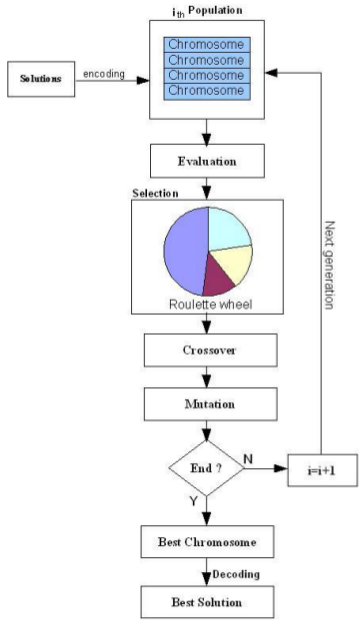
\includegraphics[scale=.7]{images/genetic_algo_flowchart.png}
			\caption{Diagramme d'un algorithme génétique standard}
			\label{fig:genetic_algo_flowchart}
		\end{center}
	\end{figure}
	
	\newpage
	
	\subsection{Les opérateurs}
		Un algorithme génétique simple utilise les trois opérateurs suivants : la sélection, le croisement et la mutation.
		\subsubsection{L’opérateur de sélection}
		L'opérateur de sélection désigne le processus par lequel les individus d'une population sont choisis en fonction de leur fonction de \emph{fitness} dans le but de former une nouvelle génération. Le choix d'un individu est proportionnel à sa fonction de fitness. Un individu avec une valeur de \emph{fitness} plus élevée aura plus de chance d’être sélectionné qu’un autre avec une valeur de \emph{fitness} inférieure. Un opérateur simple de sélection est la méthode du \emph{Roulette Wheel} ou roulette pondérée où chaque individu d’une population dispose d'une probabilité d'être choisi proportionnelle à sa valeur de fitness. Le choix des individus devant se reproduire est alors effectué sur la base de ces probabilités et est aléatoire. En effet, l'aspect aléatoire tend à protéger la population d'un manque de diversité en évitant de privilégier d'un individu ou d'un groupe d'individu sur le reste de la population.
		
	\subsubsection{L’opérateur de croisement}
	Le croisement s'applique sur deux individus. Sa principale composante est le transfert de gènes des deux individus sélectionnés dans le but de produire de nouveaux chromosomes dits chromosomes "\emph{fils}". Chacun des enfants héritent donc d'une partie du patrimoine génétique des parents. Différentes formes de croisement existent au nombre desquels nous pouvons citer:
	\begin{description}
		\item[\textsl{Le croisement à un point :}] Il consiste à désigner au hasard un point du génotype. Ce point divise donc le génotype des parents en deux parties distinctes. Ainsi, un des enfants prend une partie "\emph{avant}" d'un des parents et le recombine avec la partie "\emph{arrière}" de l'autre parent. Le second fait de même en prenant la partie "\emph{arrière}" du premier parent et le recombine avec la partie "\emph{avant}" du second parent.
		
		\item[\textsl{Le croisement à deux points :}] Le principe est le même que celui du croisement en un point sauf que deux points de croisement sont désignés ici au hasard. Ces deux points divisent le génotype des parents en trois sections qui seront transférées aux individus "\emph{fils}"
	
		\item[\textsl{Le croisement uniforme :}] Il a été proposé par Syswerda \cite{Syswerda} et consiste à désigner pour un individu "\emph{fils}" et avec la même probabilité attribuée aux gènes de l'individu parent quels sont les allèles qui lui seront transmis à leur même position dans l'individu parent.
	
	\end{description}
	
	\subsubsection{L'opérateur de mutation}
	
	La mutation est une opération qui n'intervient que sur un unique individu. La mutation consiste à altérer la valeur d'un gène pour un individu. Il s'agit d'un remplacement de la valeur d'un gène par une autre valeur. La mutation est un élément important dans la conservation de la diversité au sein d'une population. En règle général, la mutation n'intervient que très rarement et n'améliore pas le qualité d'un individu. La mutation vise à reproduire l'erreur qui survient dans le nature lorsqu'un chromosome est reproduit ou copié.
	
	\subsection{Les algorithmes génétiques parallèles}
	
	Le développement d'ordinateurs massivement parallèles et le besoin toujours plus pressant de performance dans les systèmes d'aide à la prise de décision en industrie ont amené les chercheurs à se pencher sur la problématique de l'amélioration des performances en temps et en qualité des algorithmes génétiques. Des recherches menées \cite{cant2}, trois modèles tous parallèles d'algorithmes génétiques ont émergé. L'idée derrière ces modèles est l'application du principe de "diviser pour règner". Il s'agit de diviser une tâche principale en sous-tâches à attribuer à différents processeurs. Ces trois modèles appliquent à leurs manières ce principe. Le premier modèle est le modèle des algorithmes génétiques parallèles de type \emph{master-slave}, le second est le modèle des algorithmes génétiques parallèles de type \emph{coarse-grained} et le troisième est le modèle des algorithmes génétiques parallèles génétiques parallèles de type \emph{fine-grained}.
	
	\subsubsection{Les algorithmes génétiques parallèles de type \emph{master-slave}}
	
	Les \emph{master-slave parallel genetic algorithms} (M-PGA) ou algorithmes génétiques parallèles de type \emph{master-slave} sont le type le plus simple d'algorithmes génétiques parallèles. Elles consistent essentiellement à distribuer l'évaluation de la population globale entre plusieurs processeurs. Le processeur qui conserve la population et exécute l'algorithme génétique est le maître et les processeurs qui évaluent la population sont les esclaves. La figure \ref{fig:master_slave_ga} montre un schéma de l'algorithme génétique parallèle de type \emph{master-slave}. 
	
	\begin{figure}[!h]
		\begin{center}
			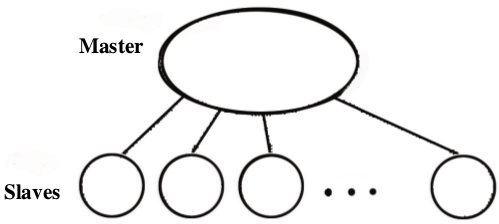
\includegraphics[scale=.3]{images/master_slave_ga.png}
			\caption{Schéma d'un algorithme génétique de type "master-slave" \cite{cant}}
			\label{fig:master_slave_ga}
		\end{center}
	\end{figure}
 
	\subsubsection{Les algorithmes génétiques parallèles \emph{coarse-grained}}
	
	Les algorithmes génétiques de type "\emph{coarse-grained}" ou encore "\emph{modèle de l'île}" consistent en un ensemble de sous-populations qui échangent des individus de manière fréquente. La complexité de ces algorithmes réside dans le fait qu'ils nécessitent de contrôler beaucoup de paramètres. Cependant, plus les sous-populations sont utilisées, plus leur taille peut être réduite sans sacrifier la qualité de la recherche. Vu que chaque processus s'exécute en parallèle, il en résulte une réduction du temps dédié aux calculs. Cependant, utiliser plus de sous-populations et donc de processus augmente la communication dans le système. Un compromis doit donc être trouvé entre le temps de calculs et le temps de communication. L'implémentation des algorithmes génétiques parallèles de type \emph{"coarse-grained"} soulève généralement trois problématiques principalement sur la migration qui est l'échange d'individus entre processus. Il s'agit de la fréquence de migration, du nombre d'individus à échanger, de la topologie des connexions entre processus et de la méthode d'intégration des migrants.\\

	\textsl{\textbf{Fréquence de migration}} \\
	La migration affecte la qualité de la recherche et l'efficacité de l'algorithme en plusieurs points. Ainsi, de fréquentes migrations entraînent l'échange massif de potentiellement bons matériels génétiques, mais il affecte aussi négativement la performance dans la mesure où les communications sont coûteuses. La même chose se produit dans les topologies densément connectées où chaque processus communique avec les autres. Le but ultime des algorithmes génétiques parallèles est de trouver de bonnes solutions assez rapidement. Il est donc nécessaire de trouver l'équilibre entre le coût de la migration et l'augmentation des chances de trouver de bonnes solutions.\\
	
	\textsl{\textbf{Choix et nombre de migrants}} \\
	La migration envoie un nombre prédéterminé d'individus d'un processus à ces processus voisins logiques sur le graphe de communications. Ces individus ou "\emph{migrants}" seront ainsi intégrés dans la population des processus auxquels ils ont été envoyés. Il est possible de choisir les "migrants" de façon aléatoire ou alors parmi les meilleurs individus de la population actuelle. La sélection aléatoire a l'avantage de disséminer plus de diversité et les chances d'explorer de nouvelles régions de l'espace de recherche peuvent être améliorées. La sélection des meilleurs individus peut aider à disséminer un matériel génétique qui a déjà été testé et qui serait donc intéressant.\\
	
	\textsl{\textbf{Topologie de connexions}}\\
	La topologie est également une importante partie des algorithmes génétiques de type \emph{"coarse-grained"}. En théorie, toutes les topologies arbitraires peuvent être utilisées. Cependant, certains modèles sont fréquents. Il s'agit : des topologies linéaires, des anneaux, des hypercubes. des densément connectés, des isolés.\\
	
	\textsl{\textbf{Méthode d'intégration des migrants}}\\
 	Différentes alternatives existent pour incorporer les "\emph{migrants}". Deux d'entre elles sont récurrentes. Il s'agit: du remplacement aléatoire des individus de la population actuelle par les "\emph{migrants}" et du remplacement compétitif ou élitiste. Dans le remplacement aléatoire, les individus devant être remplacés sont désignés de manière aléatoire. Dans le remplacement compétitif, seuls les individus avec les plus mauvais scores de "fitness" sont remplacés par les nouveaux arrivants.
	
	\subsubsection{Les algorithmes génétiques parallèles \emph{fine-grained}}
	
	Les algorithmes génétiques parallèles de type "\emph{fine-grained}" ont seulement une population, mais la structure spatiale limite les interactions entre les individus. Un individu ne peut compétir et se reproduire qu'avec ses individus voisins. Vu que les voisinages se chevauchent, les bonnes solutions peuvent ainsi se disséminer à travers la population entière. Le choix le plus important dans l'implémentation de ce type d'algorithmes génétiques parallèles est : la topologie de connexions.\\
	
	\textsl{\textbf{Topologie de connexions}}\\
	Différentes topologies de connexions sont valables. Il s'agit entre autres des grilles 2-D, des hypercubes, le torus, le cube. Il est cependant répandu de placer les individus dans un algorithme génétique parallèle de type "\emph{fine-grained}" dans une grille 2-Dimension. En effet, dans la plupart des ordinateurs massivement parallèles, les éléments de traitement et de calculs sont connectés en suivant cette topologie \cite{cant2}.\\
	
	\textsl{\textbf{Principe de fonctionnement}}\\
	Le principe de fonctionnement des algorithmes génétiques parallèles de type "\emph{fine-grained}" est différent de celui de type \emph{coarse-grained} et \emph{master-slave} et est détaillé à l'algorithme \ref{alg:principe_fine_grained}. \\
	\\
	\begin{algorithm}[H]
 		\caption{Principe des algorithmes génétiques parallèles de type "\emph{fine-grained}" \cite{nayak}}
 		\label{alg:principe_fine_grained}
 		\BlankLine
 		\For{chaque nœud en parallèle}{
 		generer un individu de façon aléatoire
 		}
 		\BlankLine
 		\While{le critère de terminaison n'est pas satisfait}{
 			\For{chaque nœud en parallèle}{
 			evaluer le fitness de l'individu \\
 			obtenir la valeur de fitness des individus voisins \\
 			selectionner l'individu voisin dont la valeur de fitness est la plus grande \\
 			appliquer un croisement avec cet individu \\
 			muter l'individu qui en a résulté \\
 			}
 			Tester le critère de terminaison
 		}
	\end{algorithm}
	
	\subsubsection{Hiérarchisation entre algorithmes génétiques parallèles}{\label{sec:algo_hierarchique}}
	
	\textsl{\textbf{Algorithme génétiques parallèles et hiérarchiques entre \emph{coarse-grained} et \emph{master-slave}}}\\
	
	\hspace*{.5cm} Une fois, ces différents modèles d'algorithmes génétiques parallèles abordés, la question de l'implémentation rapide des algorithmes génétiques parallèles de type \emph{coarse-grained }revient. Une des réponses serait en effet de combiner ces algorithmes génétiques parallèles avec les algorithmes génétiques parallèles de type \emph{master-slave} par exemple. On obtient alors une nouvelle classe d'algorithmes génétiques parallèles que sont les algorithmes génétiques parallèles hiérarchiques\cite{cant2} avec au niveau supérieur un algorithme génétique parallèle de type \emph{coarse-grained} et au niveau inférieur un algorithme génétique parallèle de type \emph{master-slave} comme le présente la figure \ref{fig:hierarchical_gene1_fig}. \\
 	
	\begin{figure}[!h]
		\begin{center}
			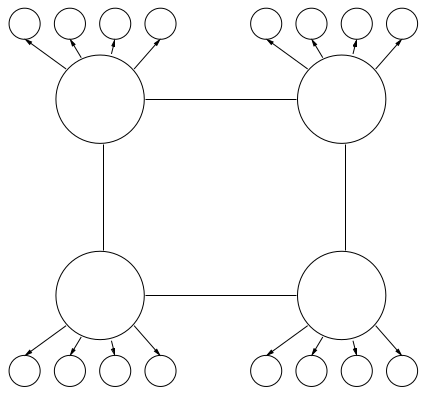
\includegraphics[scale=.3]{images/hierarchical_gene1_fig.png}
			\caption{Algorithmes génétiques parallèles et hierarchiques avec au niveau supérieur un algorithme génétique parallèle de type \emph{coarse-grained} et au niveau inférieur un algorithme génétique parallèle de type \emph{master-slave} \cite{cant2}}
			\label{fig:hierarchical_gene1_fig}
		\end{center}
	\end{figure} 	
	
	\textsl{\textbf{Algorithme génétiques parallèles et hiérarchiques entre \emph{coarse-grained} et \emph{fine-grained}}}\\
	
	Des chercheurs \cite{cant2} ont combiné deux des modèles d'algorithmes génétiques parallèles produisant des algorithmes génétiques parallèles hiérarchiques. Il s'agit des algorithmes génétiques parallèles de type \emph{coarse-grained} et de type \emph{fine-grained}. Ce nouvel algorithme ajoute un nouveau degré de complexité à ces algorithmes déjà compliqués. On obtient alors des algorithmes génétiques parallèles hiérarchiques avec au niveau supérieur un algorithme génétique parallèle de type \emph{coarse-grained} et au niveau inférieur un algorithme génétique de type \emph{fine-grained} comme détaillé à la figure \ref{fig:hierar_fine_grained_fig}.
	
	\begin{figure}[!h]
		\begin{center}
			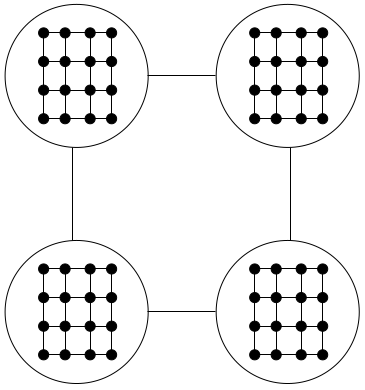
\includegraphics[scale=.3]{images/hierar_fine_grained_fig.png}
			\caption{Hiérarchie entre algorithmes génétiques parallèles de type \emph{fine-grained} et de type \emph{coarse-grained} \cite{cant2}}
			\label{fig:hierar_fine_grained_fig}
		\end{center}
	\end{figure} 
	
	\subsubsection{Hybridation}
	
	L'hybridation \cite{Goncalves} consiste à combiner deux méthodes de recherche afin d'engendrer une nouvelle méthode de recherche dit \emph{hybride}. Les algorithmes génétiques facilitent l'hybridation avec les autres techniques de recherche locale afin d'obtenir la solution optimale. De façon basique, la recherche locale et les algorithmes génétiques sont complémentaires. Les algorithmes génétiques sont efficaces lorsqu'il s'agit de parcourir un espace de recherche global, dans la mesure où elles sont capables de rapidement trouver des régions prometteuses. Cependant, elles prennent relativement beaucoup de temps à trouver des optimums dans ces régions. La recherche locale est capable de trouver des optimums avec une grande précision.
	
	\subsection{Application des algorithmes génétiques aux problèmes d'optimisation}
	
	Les algorithmes génétiques ont fait l'objet de différentes études ces dernières années \cite{jawahar}. Ils ont montré leur efficacité sur des problèmes combinatoires tels que les problèmes d’ordonnancement \cite{davis} et les problèmes de collecte et de distribution. Les algorithmes génétiques ont été testés et ont permis notamment de résoudre les problèmes d’ordonnancement d’un atelier classique de type Job-Shop (JSP). \cite{boukef}. Des algorithmes hybrides ont aussi été appliqués avec succès sur des problèmes d'optimisation. \cite{cavalieri}. La représentation du génotype reste une problématique importance dans la résolution de ces problèmes. Différentes approches de représentation et différents types d’opérateurs d’AGs ont été proposés, pour résoudre ces problèmes \cite{suer}.
	
	\section*{Conclusion}
	\addcontentsline{toc}{section}{Conclusion}
	Le dimensionnement de lots en planification de production est un important défi pour les entreprises industrielles. Il consiste à trouver un plan de production qui satisfait aux contraintes spécifiques relatives au système de production. Le PSP constitue en effet une variante NP-Difficile de ces types de problèmes. Plusieurs méthodes peuvent servir à résoudre ce problème. Au nombre de ces méthodes, figurent les algorithmes génétiques. Les AGs, à travers l'exploration et l'exploitation de l'espace de recherche ont permis de résoudre bon nombre de problèmes d'optimisation par le passé. Nous avons également présenté le PSP ainsi que les modèles et leur formulation qui ont été utilisés dans sa résolution.	Dans le partie suivante, nous décrivons les outils de test, les méthodes de résolution proposées ainsi que les algorithmes associés.
